 \section{Evaluation}\label{sec:eval}

 We implement three representative applications, as described in
 Section~\ref{sec:scenarios}, using either \conesc or nesC. The
 implementations are functionally equivalent. Based on these, we
 evaluate our approach along four key
 dimensions. Section~\ref{sec:evalcomp} analyzes the severity of
 different \emph{coupling types} in our implementations. Tighter forms
 of coupling are generally detrimental to code maintenance and
 evolution~\cite{koopman10:better}. Section~\ref{sec:complexity}
 reports code metrics assessing the \emph{complexity} of the resulting
 implementations, which often impacts a system's reliability and ease
 of debugging~\cite{koopman10:better}. The efforts required for
 evolving the software are measured in Sec.~\ref{sec:evolve} based on
 representative case studies.  Finally, Section~\ref{sec:overhead}
 quantifies the performance overhead, in terms of MCU and memory
 penalty, incurred when using \conesc.

% Overall, our evaluation reveals that:\lm{Whenever space allows, it's
%   useful to summarize the major outcomes of an evaluation
%   section. Let's see if we manage to keep it.}
% \begin{enumerate}
% \item ...
% \end{enumerate}

% In this section we show the evaluation of our approach. To this end, we
% developed several scenarios for WSNs and compare nesC implementations against
% its ConesC-written analogs. In addition to the main motivating example shown
% in Sec.~\ref{sec:appdesign}, we describe two more applications for WSNs.

\subsection{Applications}\label{sec:scenarios}

To demonstrate the generality of our design, we implement a smart-home
controller and an adaptive protocol stack in addition to the wildlife
tracking application.

The smart-home controller, whose design is shown in
Fig.~\ref{fig:shd}, relies on context information to regulate
temperature and lighting conditions in a room, as well as to deal with
emergency situations. The former functionality are driven by
user-provided preferences that depend on the current context. The
preferences are managed within the \emph{Preferences} group, whose
contexts provide different operating parameters depending on day/night
and working days vs.\ weekend conditions. The context transitions
within the \emph{Light} and \emph{Temperature} groups are driven by
thresholds found in such parameter set, compared against current
temperature and light readings. When transitioning between these
contexts, the node operates actuators to control the HVAC and lighting
systems. The controller exploits image, fire, and smoke sensors to
detect housebreaking and fire situations. It may notify the user about
the incident and possibly relay data to a controller in a different
room, depending on the situation.

% The diagram on  displays the possible application of a
% Smart-Home scenario, where each room is supplied with one node. The latter
% detects a \emph{Light} and \emph{Climate} by using corresponding
% sensors. The node uses actuators to adjusts the luminosity and climate according
% to thresholds given by current \emph{Preferences}. The latter depends on the
% time of the day and the day of the week.

% System scenario has CTP backbone and mobile/static nodes around it

\putfigure{caption=Smart-home controller context diagram.,label=fig:shd}{
 \centering
 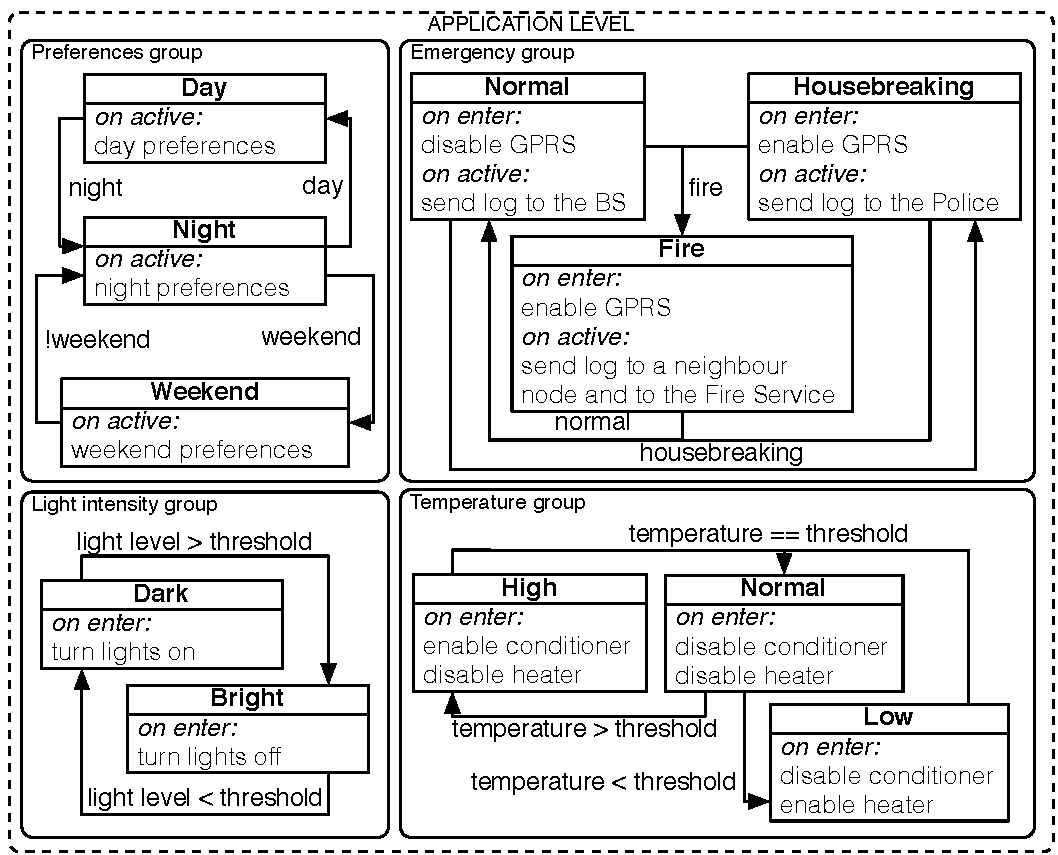
\includegraphics[width=\columnwidth]{pdf/smarthome}
}

The adaptive protocol stack, whose detailed context diagram we omit
for brevity, implements a dynamic protocol switching functionality in
situations where a node may alternative periods of significant
mobility to periods of static operation. The node roams within a
network of static nodes running CTP~\cite{gnawali09}. As long as the
node remains static, it joins the existing routing tree by running an
instance of CTP. As soon as the on-board accelerometer detects a
significant movement, it switches to a route-less gossip protocol,
which allows the node to relay data to the static infrastructure
opportunistically~\cite{Fotouhi:2012:SRH:2187181.2187193}. In
addition, the node may switch between three parameter sets for CTP,
depending on context information that determine whether lifetime,
bandwidth, or latency is to be favored.

% Another scenario - a system-level adaptation - is shown on Fig.~\ref{fig:apd}.
% If the network is static, it is feasible to use a \emph{Collection Tree
% Protocol}. In mobile network, however, a \emph{Gossip}-based protocol shows
% better results. Orthogonally to the \emph{Protocol type}, developer may want to
% adjust the \emph{Protocol parameters} to enhance a link quality between nodes,
% increase the lifetime of the network or use the bandwidth more effectively.

% \putfigure{caption=Adaptive protocol diagram.,label=fig:apd}{
%  \centering
%  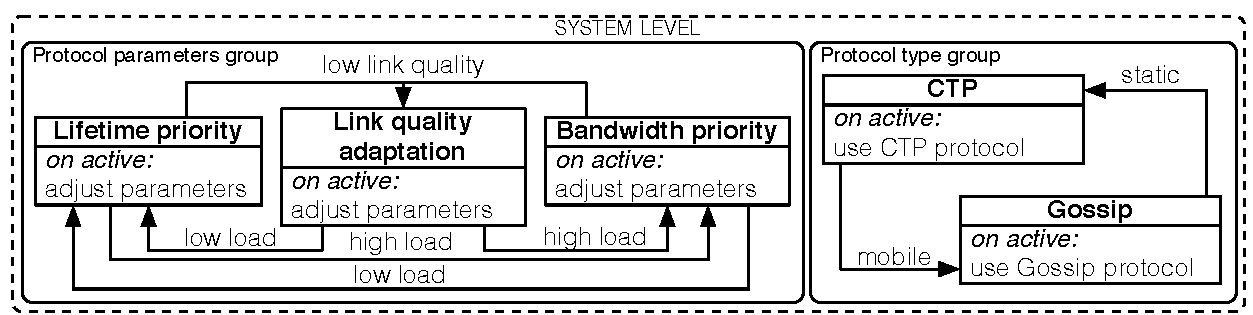
\includegraphics[width=\columnwidth]{pdf/system-level}
% }

\subsection{Coupling}\label{sec:evalcomp}

According to Stevens et al.~\cite{stevens79}, seven types of coupling
between software modules exist, as summarized in
Table~\ref{tab:couptypes}. It is generally known that the tightest is
coupling, the more difficult is debugging, maintaining, and extending
the implementations. % Coupling types, which
% are presented in this section, are not forbidden in ConesC, but some
% of them can be easily avoided with a proper use of its concepts.
We investigate the types of coupling we can observe in \conesc and
nesC implementations.

\fakepar{Results} Table~\ref{tab:coupres} illustrates the results of
our analysis. Generally, the ConesC implementations are significantly
more decoupled compared to their nesC counterparts. \conesc avoids
\emph{Content} coupling in that different behavioral variations are
encapsulated in different contexts. NesC programmers, on the other
hand, cannot dynamically bind command calls or event signals to
different modules, which forces them to expose internal module
information that make one module's operation depending on that of
several others'. For the same reason, nesC programmers are forced to
use global state to switch between different functionality depending
on the situation. This creates \emph{Common} coupling that is not
found in \conesc, in that the necessary functionality is automatically
generated by our translator. Finally, \conesc spares \emph{Control}
coupling as well. This is a result of allowing dynamic binding across
modules driven by the context transitions. Such functionality needs to
be hand-coded in nesC.

\begin{table}[!tb]
\renewcommand{\arraystretch}{1.3}
\caption{Coupling types.}
\vspace{-2mm}
\label{tab:couptypes}
\centering
\begin{tabular}{|l|p{2.5in}|}
\hline
\bfseries Type & \bfseries Description\\
\hline
Content (tightest) & One module relies on the internal working of another. Chang- ing one module requires changes in the other as well.\\
\hline
Common & Two or more modules share some global state, e.g., a variable.\\
\hline
External & Two or more modules share a common data format.\\
\hline
Control & One module controls the flow of another, e.g., passing infor- mation that determine how to execute.\\
\hline
Stamp & Two or more modules share a common data format, but each of them uses a different part with no overlapping.\\
\hline
Data & Two or more modules share data through a typed interface, e.g., a function call.\\
\hline
Message (loosest) & Two or more modules share data through an untyped inter- face, e.g., via message passing.\\
\hline
\end{tabular}
\vspace{-2mm}
\end{table}

\begin{table}[!tb]
\renewcommand{\arraystretch}{1.3}
\caption{Coupling comparison: \emph{\conesc implementations save most types of coupling that are unavoidable in nesC.}}
\vspace{-2mm}
\label{tab:coupres}
\centering
\begin{tabular}{|l|l|l|l|l|l|l|l|}
\hline
\bfseries Application & \rotatebox{90}{\bfseries Content} & \rotatebox{90}{\bfseries Common} 
& \rotatebox{90}{\bfseries External} & \rotatebox{90}{\bfseries Control}
& \rotatebox{90}{\bfseries Stamp} & \rotatebox{90}{\bfseries Data}
& \rotatebox{90}{\bfseries Message}\\
\hline
\hline
Wildlife tracking -- nesC &
yes&yes&yes&yes&--&yes&--\\
\hline
Wildlife tracking -- ConesC &
--&--&yes&--&--&yes&--\\
\hline
\hline
Smart-home -- nesC &
yes&yes&yes&yes&--&yes&--\\
\hline
Smart-home -- ConesC &
--&--&yes&--&--&yes&--\\
\hline
\end{tabular}
\vspace{-4mm}
\end{table}


% Implementation of context components in ConesC, example of which are presented in Fig.~\ref{fig:cc} and~\ref{fig:irc}, do not rely on internal work of each other, so the are not coupled in the sense of~\emph{Content coupling}, as compared to nesC-written application, where all the behavioral variations are encapsulated in one module or function. Since each context represents a separate state of the environment or the device the system operates in, contexts are not intended to share any global states, to control the flow of each other and to pass the information how to execute. Our abstraction toward~\emph{context
% groups} allows developers to perform system-level operations -- e.g. data storage --
% orthogonally to the data processing without actual modules coupling involved.


However, both \conesc and nesC force~\emph{Data} and~\emph{External}
couplings. This is unavoidable, in that both rely on typed interfaces
and different modules in both implementations must necessarily agree
on a common data format.
% We did not use, however, neither messages to share data
% nor different parts of the same data format, so~\emph{Stamp}
% and~\emph{Message} couplings are avoided in both implementations.


\subsection{Complexity}\label{sec:complexity}

We estimate the complexity of the implementations by measuring the
number of variable declarations and the number of functions in every
module. These are generally considered as intuitive indicators of a
program's complexity~\cite{koopman10:better}. It is also observed that
complexity is a function of the number of states in which the program
can find itself~\cite{koopman10:better}. A state here is any possible
assignment of values to the program variables. Thus, the number of
states must be computed by looking at the different combinations of
values assumed by variables during every possible execution.

To carry out the latter analysis, we use
SATABS~\cite{clarke05:satabs}, a model-checking tool for C
programs. SATABS performs off-line verification of C programs against
user-provided assertions. To do so, it searches through the relevant
program executions to check whether the assertion always holds. At the
end of the process, SATABS returns the number of states it explores in
the program.  Using a specific configuration, it is possible to force
SATABS to explore \emph{all} program executions. If the procedure
terminates, SATABS returns the total number of distinct states in a
program. We use SATABS on a per-function basis, implementing empty
stubs to replace code that we cannot process with SATABS, e.g.,
hardware drivers.

\begin{table}[!tb]
\renewcommand{\arraystretch}{1.3}
\caption{Complexity comparison: \emph{\conesc yields simpler implementations that are easier to debug and to reason about.}}
\vspace{-2mm}
\label{tab:compres}
\centering
\begin{tabular}{|l|c|c|c|c|c|c|}
\hline
&&&& \multicolumn{3}{@{\hspace{0.3em}}c@{\hspace{0.3em}}|}
{\bfseries Average per-module}\\[0.1in]
\bfseries Application & \rotatebox{90}{\bfseries LOC} 
& \rotatebox{90}{\pbox{0in}{\bfseries Variable\\declarations}} 
& \rotatebox{90}{\bfseries Functions} & \rotatebox{90}{\bfseries LOC}
& \rotatebox{90}{\pbox{0in}{\bfseries Variable\\declarations}}
& \rotatebox{90}{\bfseries Functions}\\
\hline
\hline
Wildlife tracking -- nesC&456&17&19&48&6&8\\
\hline
Wildlife tracking -- ConesC&539(440)&17&30&26,5&3&2\\
\hline
Wildlife tracking -- generated&1628&--&--&--&--&--\\
\hline
\hline
Smart-home -- nesC&360&24&28&28&2&2\\
\hline
Smart-home -- ConesC&382(289)&24&56&13&0,8&1,9\\
\hline
Smart-home -- generated&1310&--&--&--&--&--\\
\hline
\hline
Adaptive protocol -- nesC&150&10&13&38&2,5&3,25\\
\hline
Adaptive protocol -- ConesC&191(147)&5&21&14,7&0,4&1,6\\
\hline
Adaptive protocol -- generated&636&--&--&--&--&--\\
\hline
\end{tabular}
\vspace{-2mm}
\end{table}

\fakepar{Results} Table~\ref{tab:compres} illustrates our results. On
a per-module basis, \conesc shows significant reductions in both the
number of declared variables and defined functions. This comes from
the ability to dynamically bind a function call to the required
context-dependent implementation transparently to the caller. In nesC,
on the other hand, this requires defining global variables to check
what behavior needs to be triggered depending on the situation. As a
result of this, the number of per-function states programmers must
manage also drastically decreases, making the implementations simpler
to understand. % Together with the concepts of \emph{contexts}
% and~\emph{context groups}, which help in better organizing the code,
% this facilitates debugging and maintenance.

%  -- and
% boilerplate code. Because of the same reason, functions have to be
% spitted into smaller isolated parts. We believe, however, that in
% larger applications the number of the similar lines of code will be
% bigger.  

% The number of LOC can also be decreased significantly -- as
% shown in Table~\ref{tab:compres} in parentheses -- by having a tool,
% which generates a boilerplate code using a diagram of a
% context-oriented model of the application, similar to the one
% displayed in Fig.~\ref{fig:wtd}. The logical fragmentation leads to a
% code simplification, improved readability and re-useability along with
% easier debugging and maintaining processes.

As debatable as it may be for measuring the effectiveness of a
programming abstraction~\cite{mottola10:survey}, we also measured the
number of lines of code in both nesC and \conesc implementations: the
two are roughly comparable. More interestingly, however, as already
discussed, we also measured the size of the code generated by our
translator, described in Section~\ref{sec:translator}. Besides giving
an intuition of the complexity involved in the translation process,
this figure also indicates the ``expressive power'' of the
abstraction, that is, the amount of processing that \conesc
programmers can succinctly express using the language constructs we
design. As already mentioned, it turns out that the output of our
translator is roughly \emph{three times} the size of the input code,
demonstrating that our abstractions do capture a significant portion
of processing in a few simple concepts.

\subsection{Software Evolution}\label{sec:evolve}

WSN software needs to constantly evolve due to changes in
requirements. Generally, the better an implementation is modularized,
the easier are the modifications, since the changes will affect an
isolated portion of the system~\cite{koopman10:better}. For each
application we consider, we estimate the effort to modify the \conesc
implementation compared to the nesC counterpart. We study three types
of modification: removing a context, adding a new context, and adding
a new context group.

To estimate the effort for removing a context, we rework the scenario
of the adaptive protocol stack. Say developers want to remove of one
of the CTP parameter sets after testing, since those parameters
performed ineffectively. To study the addition of a new context, we
extend the wildlife tracking application to the case where it becomes
necessary to monitor the spread of a disease. To do this, developers
add a new context \emph{Carrier} to the \emph{Health conditions} group
to create a beacon for an animal who was in contact with a diseased
one, but shows no symptoms yet. To study the addition of an context
group, in the smart-home controller scenario we consider a case where
developers need to monitor a device's state depending on periodic
run-time checks. If a potential failure is discovered, the controller
should change its behavior. To this end, programmers add an entire
context group \emph{Status} with two contexts \emph{Normal} and
\emph{Failure}.

\fakepar{Results} Our analysis shows that removing a context in the
\conesc implementation of the adaptive protocol stack only requires
modifying 3 lines of code, besides deleting the context itself. To
remove unnecessary functionality in nesC, developers must modify
several lines of code scattered throughout the main module. To add a
context in the wildlife tracking application, using \conesc it is
necessary to modify 5 lines of code, besides providing the
implementation for the new context. Implementing the same extension in
nesC requires, among other code modifications, adding two new global
states, further complicating the control flow. Adding a new context
group in the smart-home controller requires modifications in about 40
lines of code using \conesc, besides providing the implementation for
the new contexts. Using nesC, about the same amount of code changes
are required, yet these include adding two global states, again
rendering the implementation necessarily more entangled. Finally,
worth noticing is that the effort to apply context-unrelated changes
in \conesc is the same as in nesC.

% as shown on Table~\ref{tab:compres}, we notice that the
% program written in context-oriented style using plane nesC is more
% than 3 times bigger than its ConesC counterpart. Our approach makes
% context-oriented programming as simple as plain nesC programming.

\subsection{MCU and memory overhead}\label{sec:overhead}

The advantages brought to programmers come at the cost of additional
system overhead. To assess this, we measure the MCU overhead for
context transitions and calls to layered functions, as well as memory
overhead when using \conesc as compared to nesC. To measure the MCU
overhead we use the MSPSim MSP430 emulator~\cite{eriksson09}, while we
estimate the memory overhead using tools in the nesC and GNU-C
toolchains. As the executions are determinstic, the run-time experiments
constantly yield the same measures.

% Since there are neither contexts nor layered functions in nesC-based
% implementation, we measured a number of CPU-cycles of parts with different
% execution flow. For example, contextual events, like a base station presence,
% are detected and handled in ConesC differently as compared to nesC, but,
% eventually, it results in the same functionality. 

\fakepar{Results} Fig.~\ref{fig:cmo} shows the results. The average
MCU overhead for a layered function call ranges from 2 to 5 MCU
cycles, depending on the application. Such figures are negligible in
terms of energy consumption, since the simplest operation in TinyOS,
that is, turning on/off an LED, already consumes 8 MCU cycles. The
overhead of context transitions is slightly larger, but in the same
order of magnitude. This arises from the activation rules, described in
Fig.~\ref{fig:ad}. Additional MCU cycles are needed to check if the transition is
possible, then to check the dependencies, and finally to execute the
body of \code{check()}. % Additionally, the overhead may grow further depending on
% the implementation of \code{activated()}/\code{deactivated()}.

Most importantly, the memory overhead is also negligible, measuring a
worst-case 2.5\% penalty for the size of the program binary and a
worst-case 4.5\% penalty for RAM usage. The complexity of the
application largely dictates the corresponding memory overhead when
using \conesc. For example, the wildlife monitoring application,
being the most complex in terms of contexts, context changes, and data
processing, shows the highest overhead.



\putfigure{caption=MCU and memory overhead: \emph{the resource usage penalty for using \conesc is almost negligible.},label=fig:cmo}{
\centering
\subfloat[MCU overhead.]{
  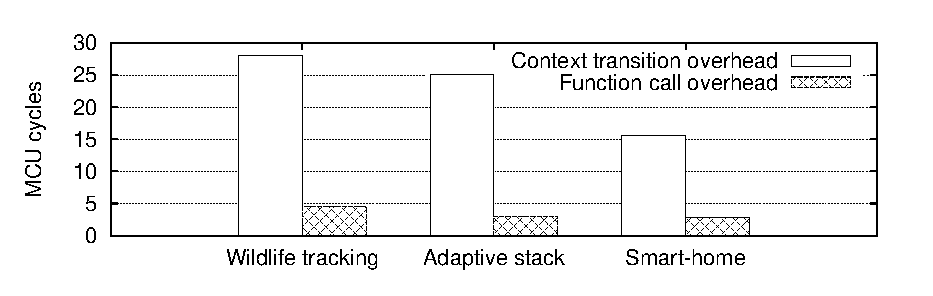
\includegraphics[width =\columnwidth]{pdf/cpu_overhead}
  \label{fig:cpuo}
}\\\vspace{-4mm}
\subfloat[Memory overhead.]{
  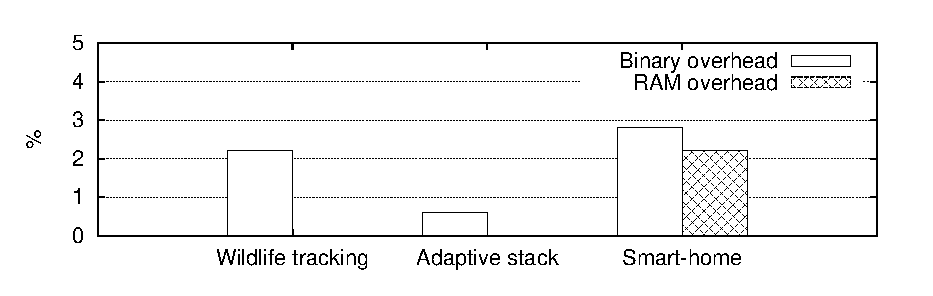
\includegraphics[width=\columnwidth]{pdf/memory_overhead}
  \label{fig:memo}
}
}


%%% Local Variables: 
%%% mode: latex
%%% TeX-master: "bare_conf"
%%% End: 
